%!TEX root = ../thesis.tex
%*******************************************************************************
%****************************** Second Chapter *********************************
%*******************************************************************************

\chapter{Systematic Uncertainties}
\label{sec:syst_uncert}

Due to the size of the available dataset, the precision of the measurement of the \ttbar cross section is dominated by systematic uncertainties and not by statistic uncertainties.
In this analysis, the systematic uncertainties are treated as nuisance parameters in a
template fit, as described in Chapter \ref{sec:xsec} . The nuisance parameters are determined in-situ allowing to reduce the impact of the systematic variations. 
Correlations between the variations are taken into account by fitting the nuisance parameters simultaneously.
The nuisance parameters are usually described by a unit Gaussian distribution describing the prior assumptions made about their behaviour.
These prior distributions (or priors) can also follow a uniform distribution depending on the specific nuisance parameter.

In this chapter the systematic uncertainties are described in detail starting with the uncertainties due to experimental effects in Section \ref{sec:exp_uncert}.
The uncertainties based on theoretical assumptions are discussed in Section \ref{sec:theo_uncert}. The treatment of the systematics as nuisance
parameters and especially the priors that are chosen to model the behaviour of the respective nuisance parameter is discussed as well.

Broadly speaking there are two ways the systematic uncertainties can change the templates: They can affect the normalization of the templates or the shape or both.
Looking in detail, most uncertainties affect both the shape and the normalization, but some clearly affect one more than the other.
An uncertainty can affect separate categories of events differently than others or affect all events similarly.
Uncertainties on the normalization of all templates are in general harder to constrain than those affecting the shape of the templates as the normalization of the
\ttbar template is directly tied to the cross section which is the parameter of interest and thus not constrained by a prior. 

All systematic uncertainties are summarised in Tabke \ref{tab:syst_sum}. The summary includes a short summary of the systematic as well as the dominant effect (normalization or shape) and
the assumed prior.

\section{Experimental Uncertainties}
\label{sec:exp_uncert}

\subsection{Uncertainties Related to the Measurement of  Leptons}

As described in Section \todo{Link}, the simulation is rescaled to model the efficiencies in data using scale factors. The efficiency measurements (expressed by the scale factors) have an uncertainty that needs to be propagated to the final measurement by varying the scale factor for the electrons or muons within its uncertainty resulting in a two sided variation.
The efficiency itself is usually measured with the Tag-and-Probe method, which allows to measure the efficiency independently in data and simulation, as described in Section \ref{sec:TriggerTPMethod}.

For the electrons, the uncertainty on the efficiency measurement is the sum of several single sources taking into account alternative models for both the background contribution
and the shape of the Z boson mass peak.
The uncertainty due to the selection of the tag lepton is evaluated by changing the selection criteria in both data and MC.
These contributions are considered to be uncorrelated and added up in quadrature. 
Since the uncertainties vary based on the kinematics of the electron, the electron effiency uncertainty also has a small shape effect on the templates for signal and background. The larger effect
is on the normalization, to the order of $\sim 0.5 \; \% - 2\; \%$ in the majority of the phase space.

In contrast, the muon efficiency uncertainty is estimated as an envelope of multiple effects. These include the binning and range that is used to model the Z boson mass peak as well as the variation of the assumed signal shape. As for the uncertainty on the electrons it also includes a change in the tag selection.
The total uncertainty is $1.25 \; \%$ independent of the muon kinematics, resulting in a pure normalization uncertainty.

The measured energy of the leptons is scaled to correct the reconstruction for possible bias, such as the reconstructed energy being larger than the original energy. In simulation the energy is smeared in addition so the energy resolution in simulation is representative of the resolution in data.
For both electrons and muons the corrections on simulation are varied to model the uncertainty.

For the electron energy, this uncertainty combines the effects of training these corrections for electrons or photons, the choice of cuts used in the training and the choice of the simulated sample that is used in the training. It also includes an uncertainty on the method itself evaluated with a closure test and a correction for a possible
dependence of the original energy of the electron.
The uncertainty on the electron energy scale and smearing are then treated as separate nuisance parameters.
The total effect follows a steeply falling function with the majority of the electrons having an energy variation in the range of $0 \; \% - 0.5 \; \%$.

For muons, the uncertainty includes changing the mass range of the Z peak as well as a statistical component. The maximum deviation of each contribution are then added in quadrature to obtain the total systematic correction.
The uncertainty on the muon energy follows a steeply falling function with the majority of the muons receiving an energy variation between $0.05 \; \% - 0.2 \; \%$.

The uncertainties on the lepton energies affect the number of selected events if an lepton has a nominal lepton \pt close to the threshold of the event selection.
Otherwise, the impact of these uncertainties should be comparatively small, as the template distributions in the fit do not directly depend on the leptons.

The systematic uncertainty on the trigger efficiency measurement is described in Section \ref{sec:TrigSF}. This uncertainty is applied by varying the respective correction scale factors
and it is correlated for all three lepton decay channels. Since it only weakly depends on the lepton kinematics it mainly has a normalization effect on the templates used in the fit.

\subsection{Uncertainties Related to Jets}

As described in Section \todo{Link} the templates used for the cross section measurement are based on jet-related observables.
Uncertainties related to jets consequently tend to directly affect the templates. However, the dependence of the total number of events on the properties of the jets is only weak in the fit,
since there are no specific requirements on jets for events in the \emu channel.

The uncertainty on the correction of the jet energy as described in Section \todo{Link to reco chapter} is split into 19 different sources depending on the $\pt$ and $\eta$ of the jets.
These sources are treated as separate uncorrelated nuisance parameters \cite{CMS-PAS-JME-16-003,Khachatryan:2016kdb}.
Similar to the nominal jet energy scale correction \todo{link to reco} the uncertainty is applied by rescaling the energy of each jet in the simulation.
These variations include the differences in the behaviour of jet fragmentation and final state radiation between Pythia6 and Herwig++ \todo{check spelling + cite}.
They also include uncertainties due to the flavor of the jet again coming from a comparison of Pythia6 and Herwig++.
Different methods to evaluate the correction of the jets themselves are compared and their difference is used as another uncertainty.
Other sources of uncertainty are the variation of the response to a single particle in both the hadronic and electromagnetic calorimeters.
The uncertainty due to the resolution of the jets is split into different regions depending on $\eta$.
The uncertainty on the estimation of pile-up is taken into account by both applying the uncertainty on the pile-up correction (see Section \todo{Link to Reco section}) in simulation and comparing simulation with and without added pile-up.
Finally the dependence on changing conditions during data taking is taken into account by applying differences between corrections limited to a certain run period and the total average correction as uncertainties.
The total uncertainty on the jet energy scale combining all the sources is in the range of $1\; \%  - 2\; \%$ in the phase space used in this measurement.

The jets in simulation are corrected to match the resolution of the jet energy in data \todo{Link to reco}. The uncertainty depends on the $\eta$ of the jet and on
the $\pt$ of the generated jet (before detector reconstruction). 
The uncertainty on the correction is applied to each jet separately by repeating the resolution correction with a changed scale factor.
This scale factor is not applied to the jet energy, but to the relative difference between the reconstructed jet and the jet at generator level.
The uncertainty on this scale factor is in the range of $\sim 1 \; \%$ in the barrel region and around $3.5 \; \% - 5 \; \%$ in the endcap region of the detector.
This uncertainty is applied 
In general, the impact of this uncertainty is lower than the impact 
of the uncertainty on the jet energy scale corrections.

The systematic uncertainty on the efficiency to correctly identify a jet originating from a b quark as a b-tagged jet is taken from a dedicated and unrelated measurement of the b-tag efficiency \todo{cite} using di-jet events. It is applied by reweighting simulated events according to this uncertainty. The uncertainty generally depends on $\pt$ and $\eta$ of the jet.
Various sources of uncertainty are taken into account like the uncertainty on the simulation of B meson fragmentation, gluon splitting and further meson branching fractions.
Furthermore, experimental uncertainties like the impact of the jet energy scale are including by propagating them to the b-tagging efficiency. The uncertainty introduced through pile-up is evaluated by propagating the uncertainty
on the pile-up determination to the b-tagging efficiency measurement.
The uncertainty on the b-tagging efficiency is on the order of $2 \; \% - 6 \; \%$ in the bulk of the measured phase space.

The uncertainty on the probability that a jet originating from a light quark could be b-tagged is treated in a similar way.

The effect of the uncertainty on the b-tagging efficiency is well visible in the multiplicity of b-tagged jets in each event shown in Figure \ref{fig:control_var_BTAGH}, especially in the ratio between the data and predicition.
It also shows that the variation on the predicted number of events is larger than the statistical uncertainty on the amount of measured events, indicating that this variation is constrained in the
template fit.

\begin{figure}[htbp!]
  \begin{center}
      \resizebox{0.48 \textwidth}{!}{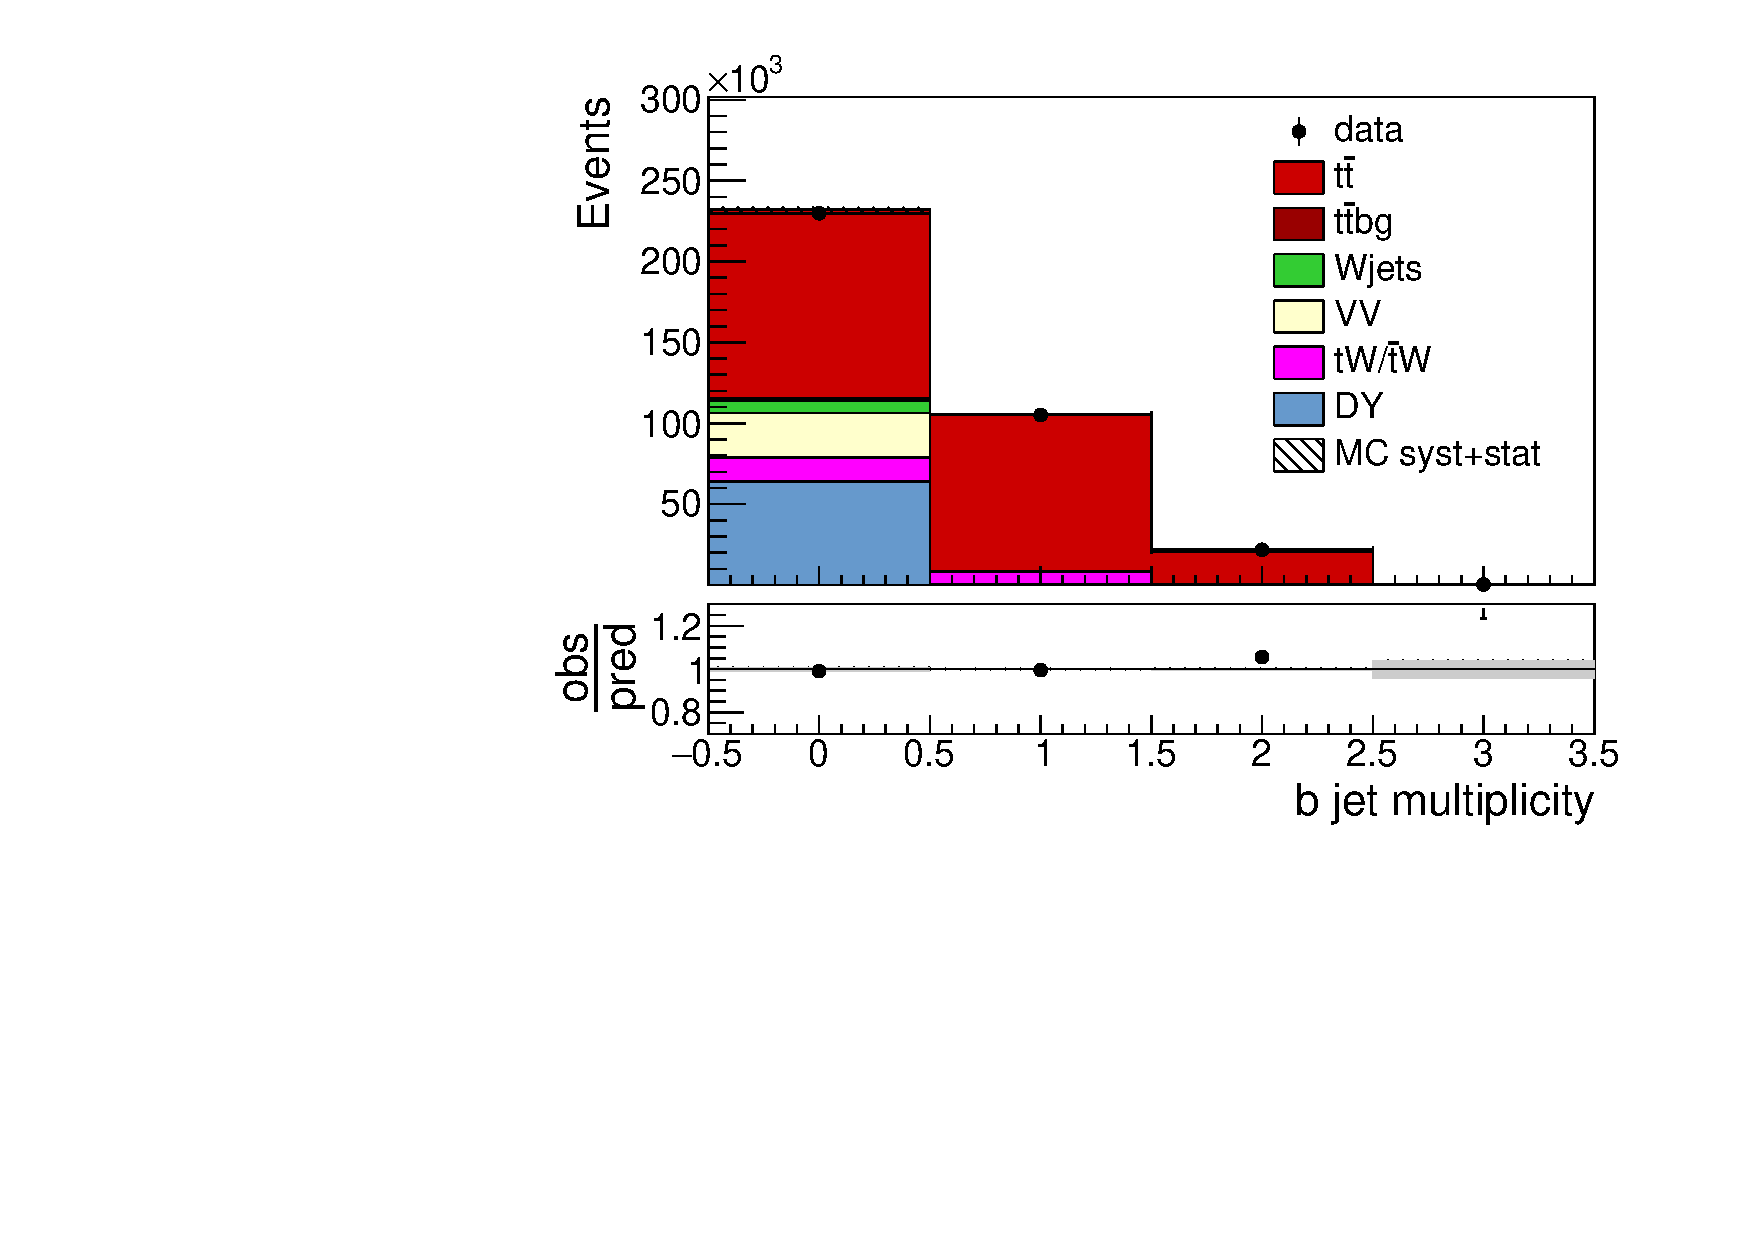
\includegraphics{SystematicUncerts/Figures/variationPlots/controlPlots/BTAGH/selected_b-jet_multi_step_8_BTAGH_down.pdf}}
    \resizebox{0.48 \textwidth}{!}{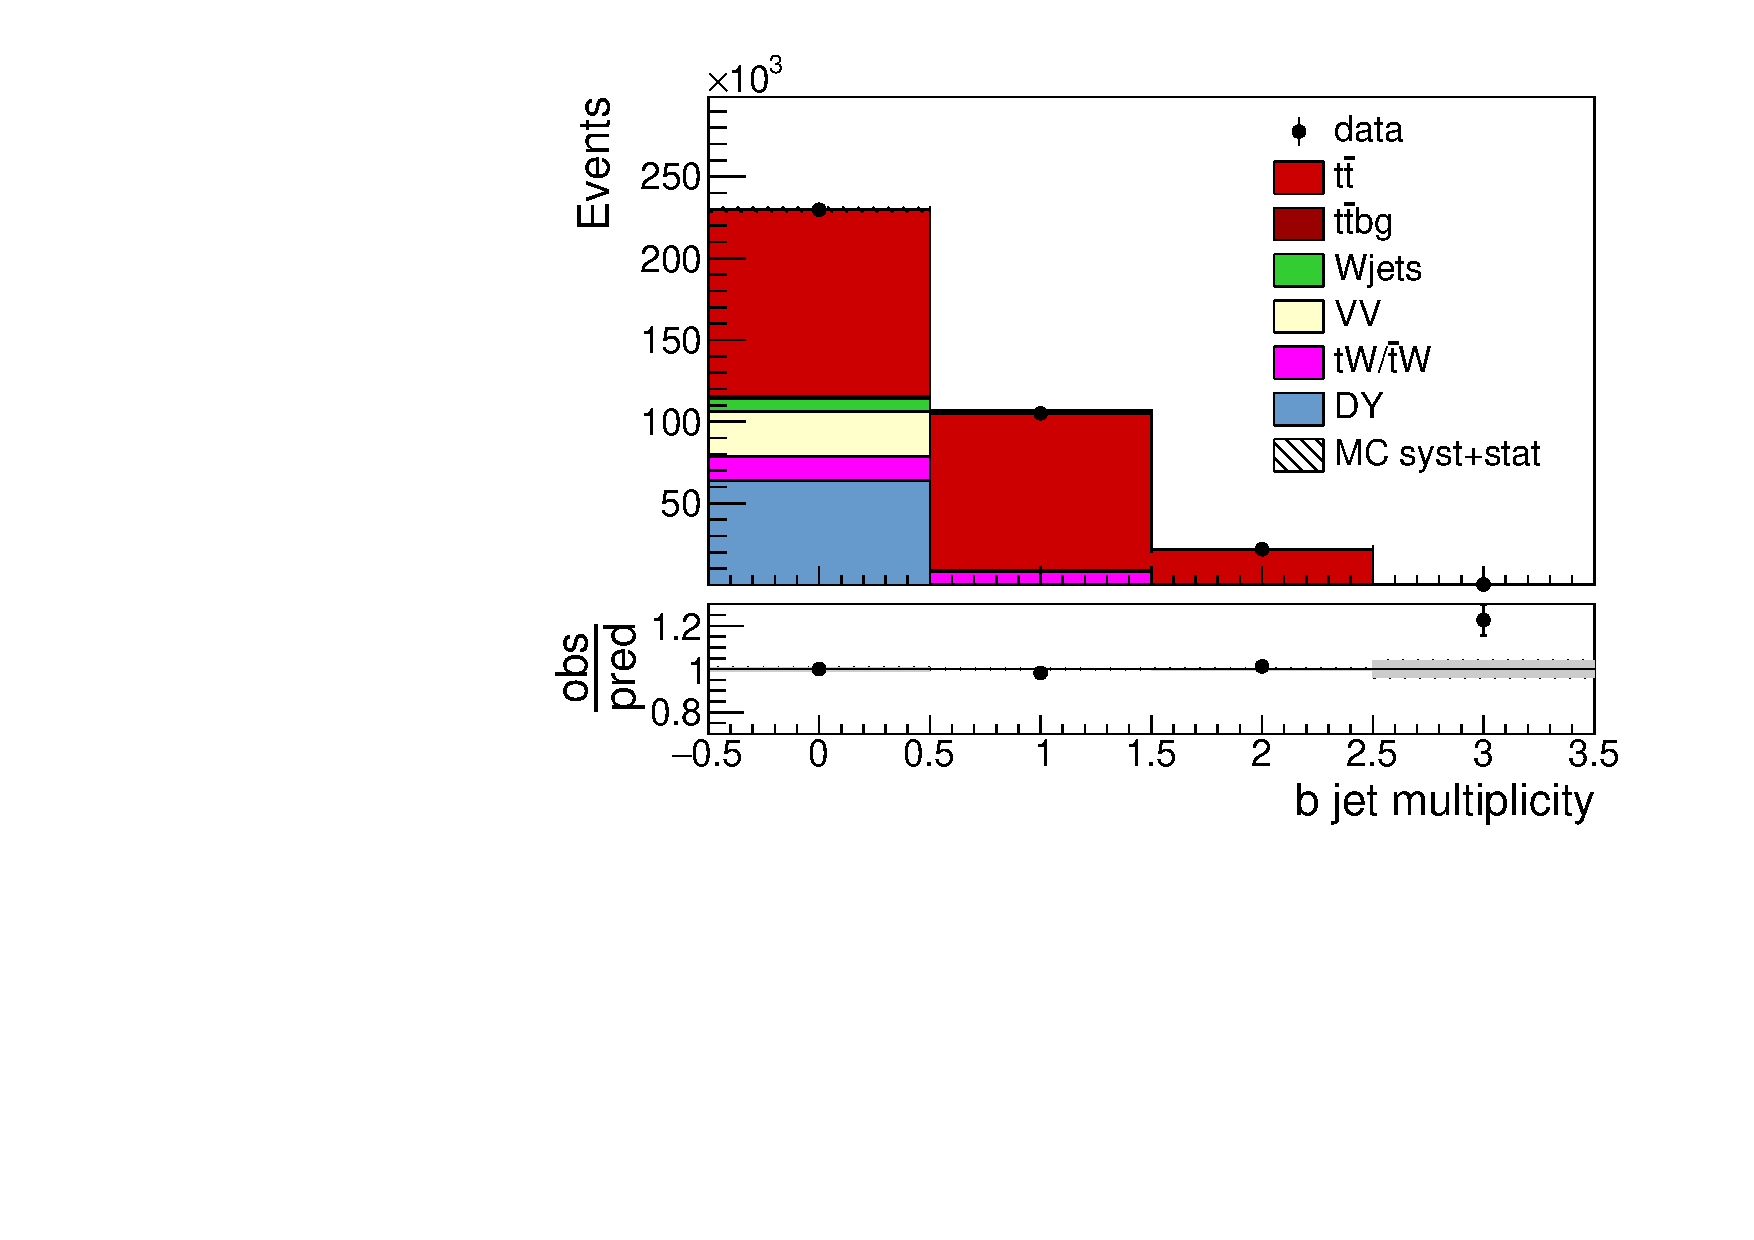
\includegraphics{SystematicUncerts/Figures/variationPlots/controlPlots/BTAGH/selected_b-jet_multi_step_8_nominal.pdf}}
    \resizebox{0.48 \textwidth}{!}{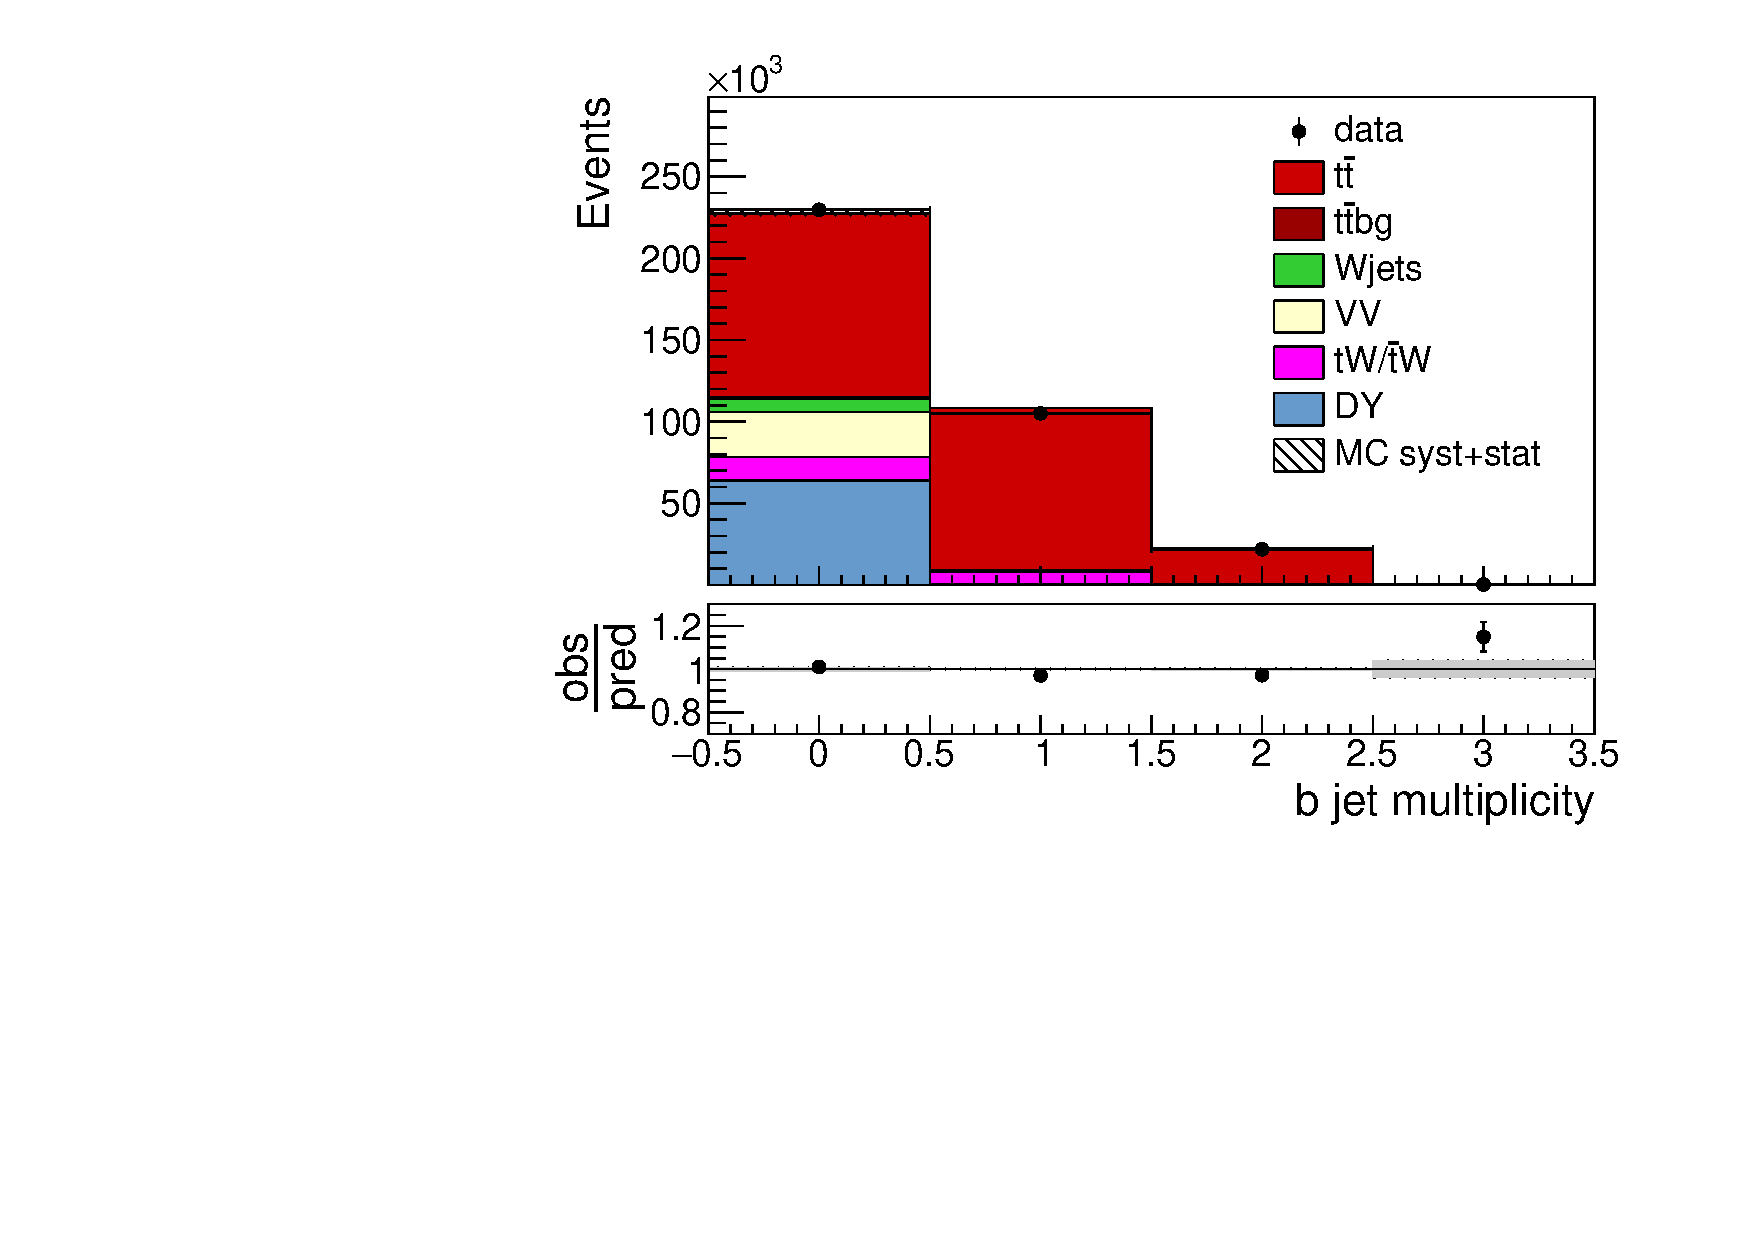
\includegraphics{SystematicUncerts/Figures/variationPlots/controlPlots/BTAGH/selected_b-jet_multi_step_8_BTAGH_up.pdf}}

\caption{Multiplicity of b-tagged jets in the \emu channel for the two systematic variations (left,right) and the nominal (middle) b-tagging efficiency.
The hatched bands correspond to the statistical uncertainty on the sum of the predicted yields. 
        The ratios of the event yield in data to the sum of the predicted yields are
        shown at the bottom of each plot. Here, the solid gray band
        represents the contribution of the statistical uncertainty.
  \label{fig:control_var_BTAGH}}
  \end{center}
\end{figure}


\subsection{Further Experimental Uncertainties}

The estimation of pile-up (see Section \todo{Link to reco}) in simulation is corrected according to the assumed number of collisions per bunch crossing in data. The number of additional collisions
in data is calculated for small time periods from the total inelastic proton proton cross section and the instantaneous luminosity in that time period.  
Events in simulation are reweighted depending on the number of primary vertices. To estimate the systematic uncertainty of this correction the total proton-proton cross section is changed
by $4.6 \; \%$ based on a measurement by the ATLAS collaboration \cite{Aaboud:2016mmw}. New eventweights are then estimated based on the changed value of the total proton-proton cross section.
The impact of these variations is shown in the distribution of the number of primary vertices per event as shown in Figure \ref{fig:control_var_PU}.
A mismatch between measured data and simulated events is visible in the nominal distribution, but as shown in the left figure, the systematic variations cover this discrapency.
This can lead to a fit result for the specific nuisance parameter tied to the systematic variation being different from one.

\begin{figure}[htbp!]
  \begin{center}
    \resizebox{0.48 \textwidth}{!}{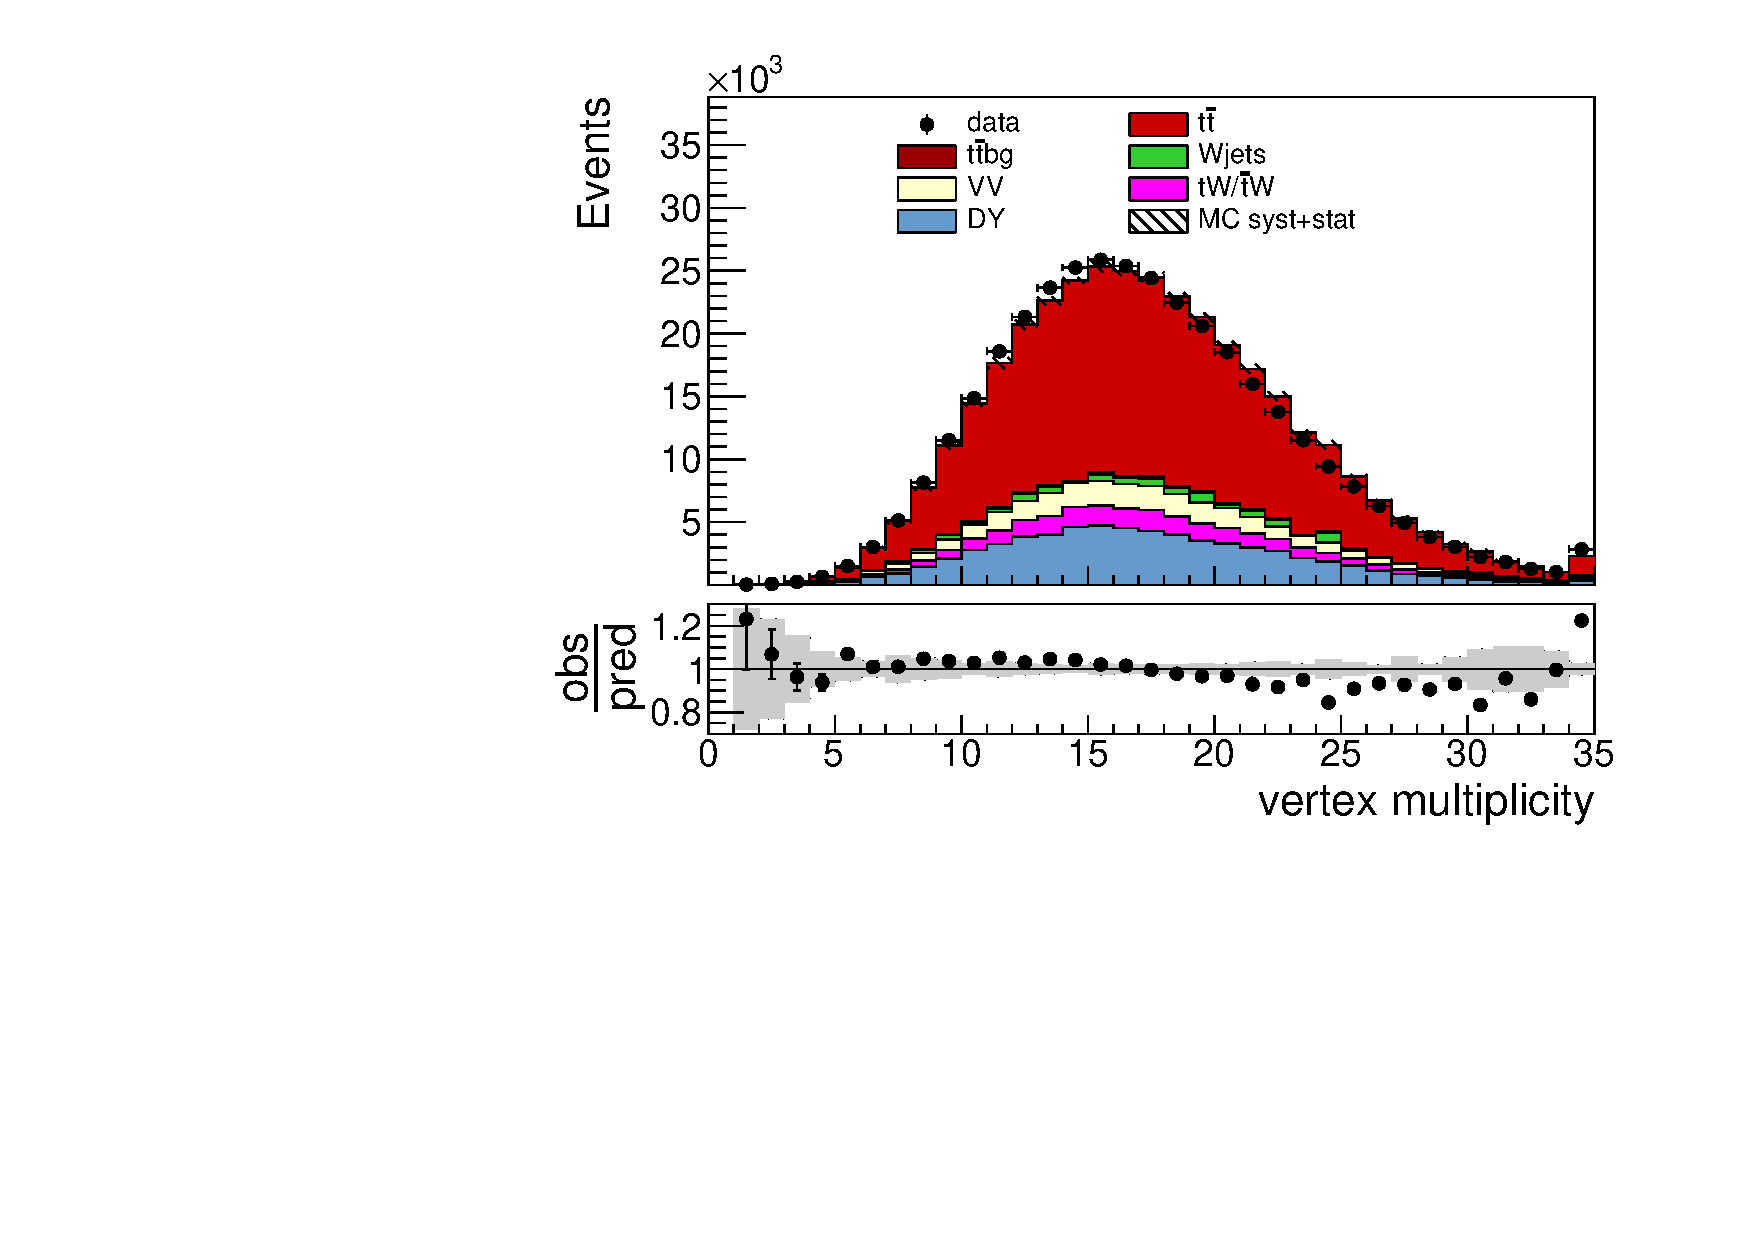
\includegraphics{SystematicUncerts/Figures/variationPlots/controlPlots/PU/vertex_multiplicity_step_8_PU_down.pdf}}
    \resizebox{0.48 \textwidth}{!}{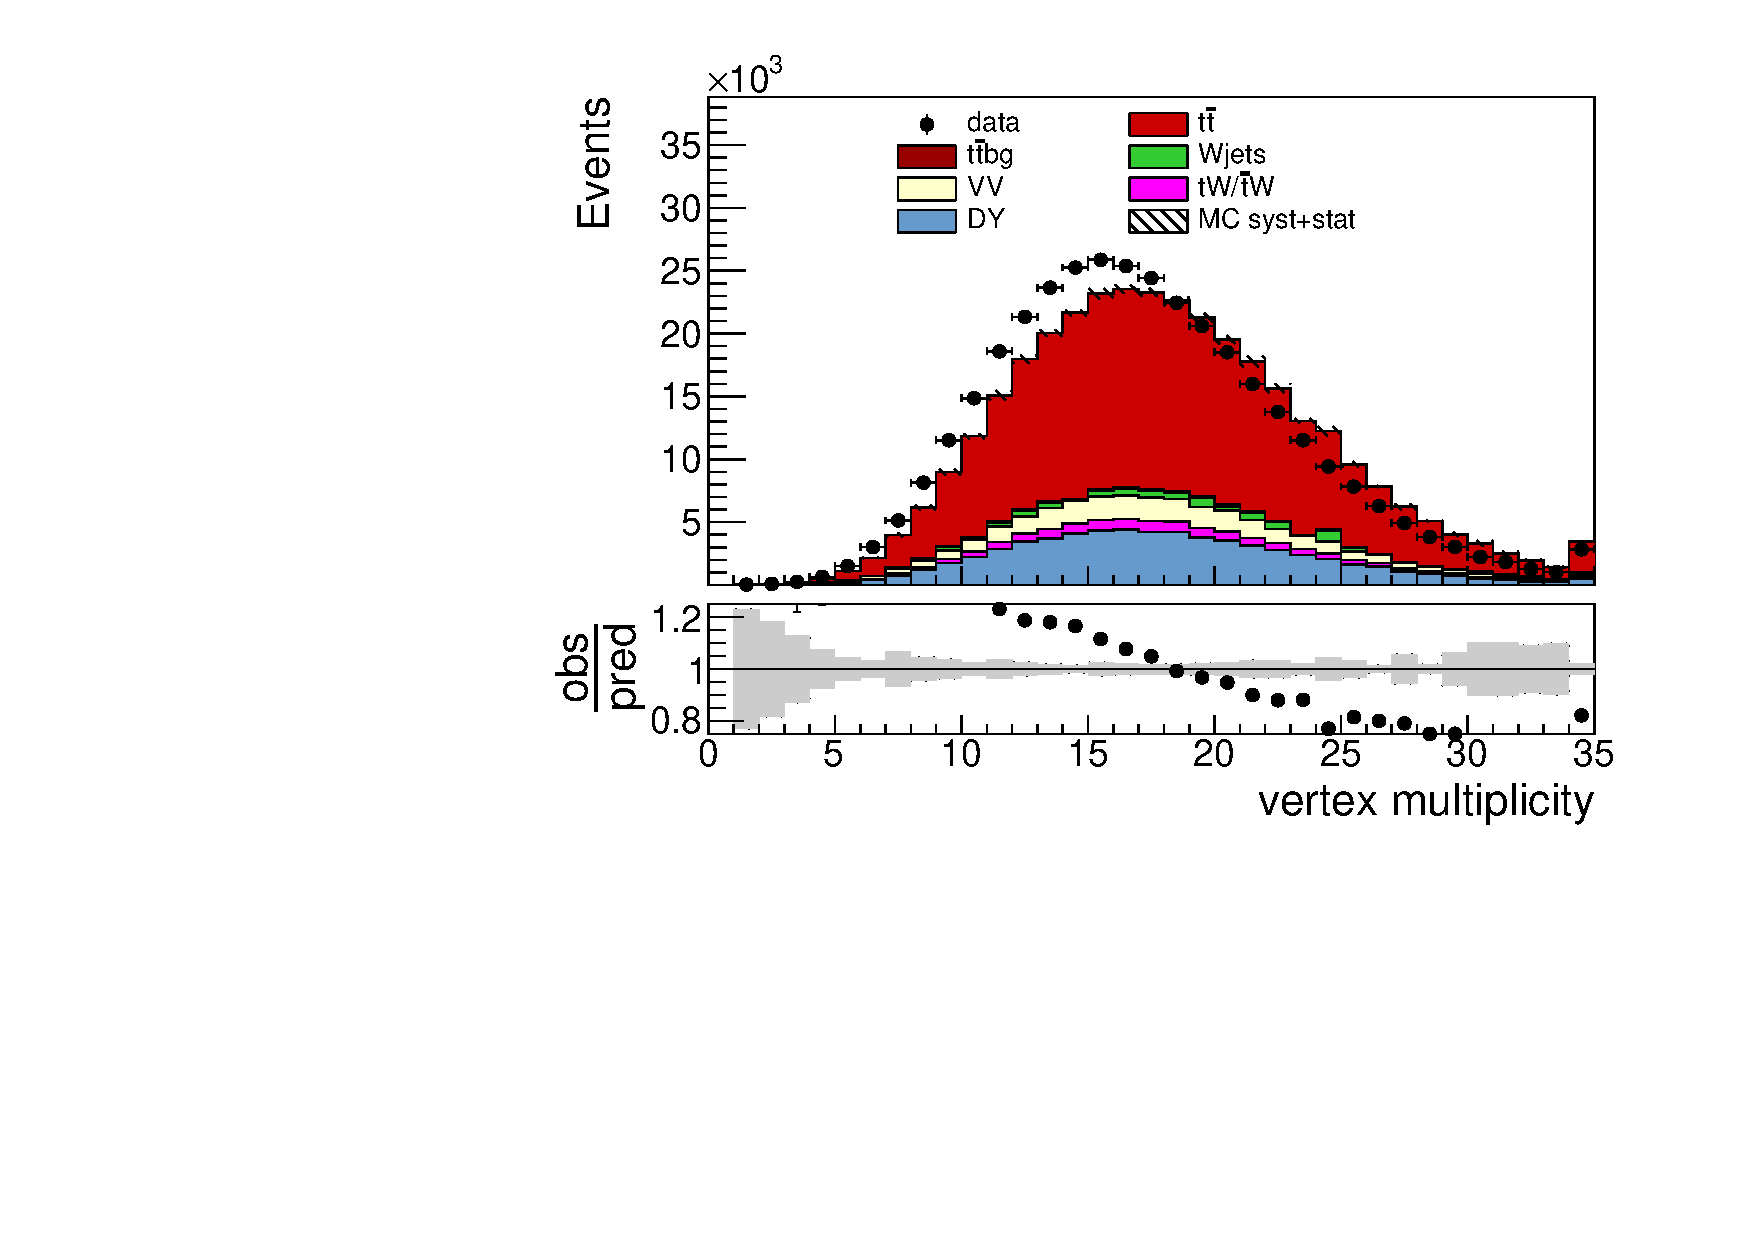
\includegraphics{SystematicUncerts/Figures/variationPlots/controlPlots/PU/vertex_multiplicity_step_8_nominal.pdf}}
    \resizebox{0.48 \textwidth}{!}{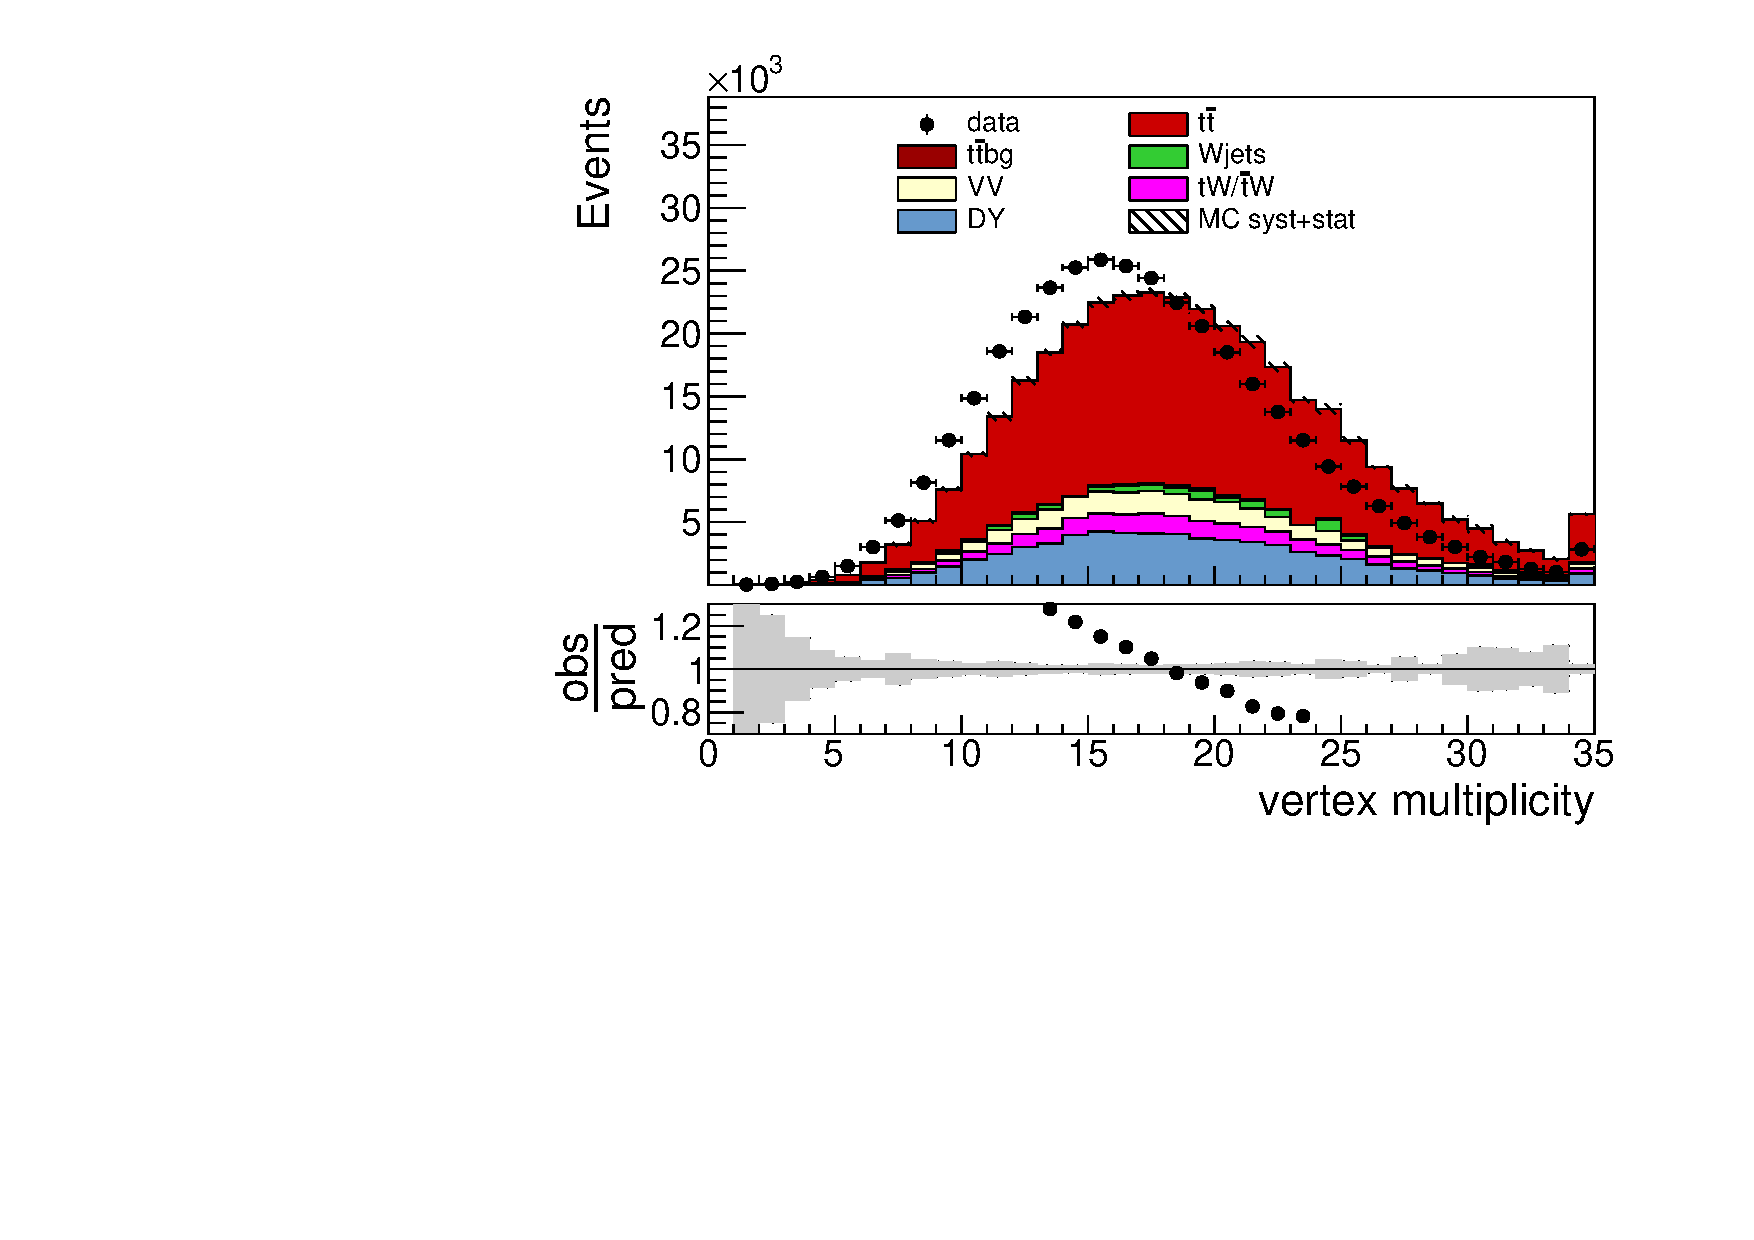
\includegraphics{SystematicUncerts/Figures/variationPlots/controlPlots/PU/vertex_multiplicity_step_8_PU_up.pdf}}
\caption{The number of primary vertices per event in the \emu channel for the two systematic variations (left,right) and the nominal (middle) pile-up corrections.
The hatched bands correspond to the statistical uncertainty on the sum of the predicted yields. 
        The ratios of the event yield in data to the sum of the predicted yields are
        shown at the bottom of each plot. Here, the solid gray band
        represents the contribution of the statistical uncertainty.
  \label{fig:control_var_PU}}
  \end{center}
\end{figure}


The integrated luminosity is determined by extrapolating the result of a measurement \todo{cite} of the instantaneous luminosity using special proton beam conditions (Van der Meer scan \cite{Zanetti:1357856}) to the full data taking period.
The uncertainty on the luminosity is determined in a dedicated analysis by both taking into account the uncertainty on the initial measurement itself as well as uncertainties
introduced in the extrapolation, mainly through changes in detector or beam conditions.
The systematic uncertainty on the luminosity is totally independent from the measurement of the \ttbar cross section and the other uncertainties described in this chapter.
It is not included as a nuisance parameter in the fit. It is directly applied to the final measurement of the \ttbar cross section by adding it in quadrature to the other uncertainties (see Equation \ref{eq:CaC})

\section{Theoretical Uncertainties}
\label{sec:theo_uncert}

The distributions used in the fit in this analysis are taken from simulation. In principle the physics model itself is not relevant, provided the simulation correctly predicts the event distribution for a given process.
The Standard Model reliably predicts the event distribution for the processes in this measurement especially for \ttbar production.
The simulation is based on assumptions for multiple parameters, some of which are based on the Standard Model. The uncertainties on the simulation are determined by the variation of these key parameters and they are
evaluated by repeating the simulation with changed parameters. The nominal simulation is then replaced with the systematically varied simulation to propagate the uncertainty to the final measurement.
The overall normalization of simulated \ttbar events is not changed with respect to the nominal sample, so the theoretical uncertainties described have a larger effect on the shape of the templates used
in the analysis than on the normalisation.

The \POWHEG simulation generates \ttbar events at NLO as described in Section \todo{Link}.
Additional particles radiated from the initial and final states are modelled in the parton shower, but the possible impact of these higher orders on the matrix element calculations is taken into account as an uncertainty.
Following convention \todo{cite smth., book from Klaus ?} the renormalization and factorisation scales are varied by the factors $2$ and $0.5$ resulting in a two-sided variation.
These variations are predicted to cover a possible change from inclusion of higher orders.
A uniform prior is used for the variation, with a value of unity between the $+1 \; \sigma$ and $-1 \; \sigma$ variations and zero everywhere else.
The impact of the matrix element scale variation is shown in Figure \ref{fig:control_var_TT_MESCALE} for the distribution of the number of jets for events with one b-tagged jet for events in the \emu channel.
These scale variations mostly affect the jets originating from particles simulated in the matrix element calculations, which often correspond to the three jets with the highest reconstructed $\pt$.
The $\pt$ of the jets is influenced by the scale and this change of $\pt$ propagates to the number of reconstructed jets due to the $\pt$ requirement in the selection of jets.

\begin{figure}[htbp!]
  \begin{center}
     \resizebox{0.48 \textwidth}{!}{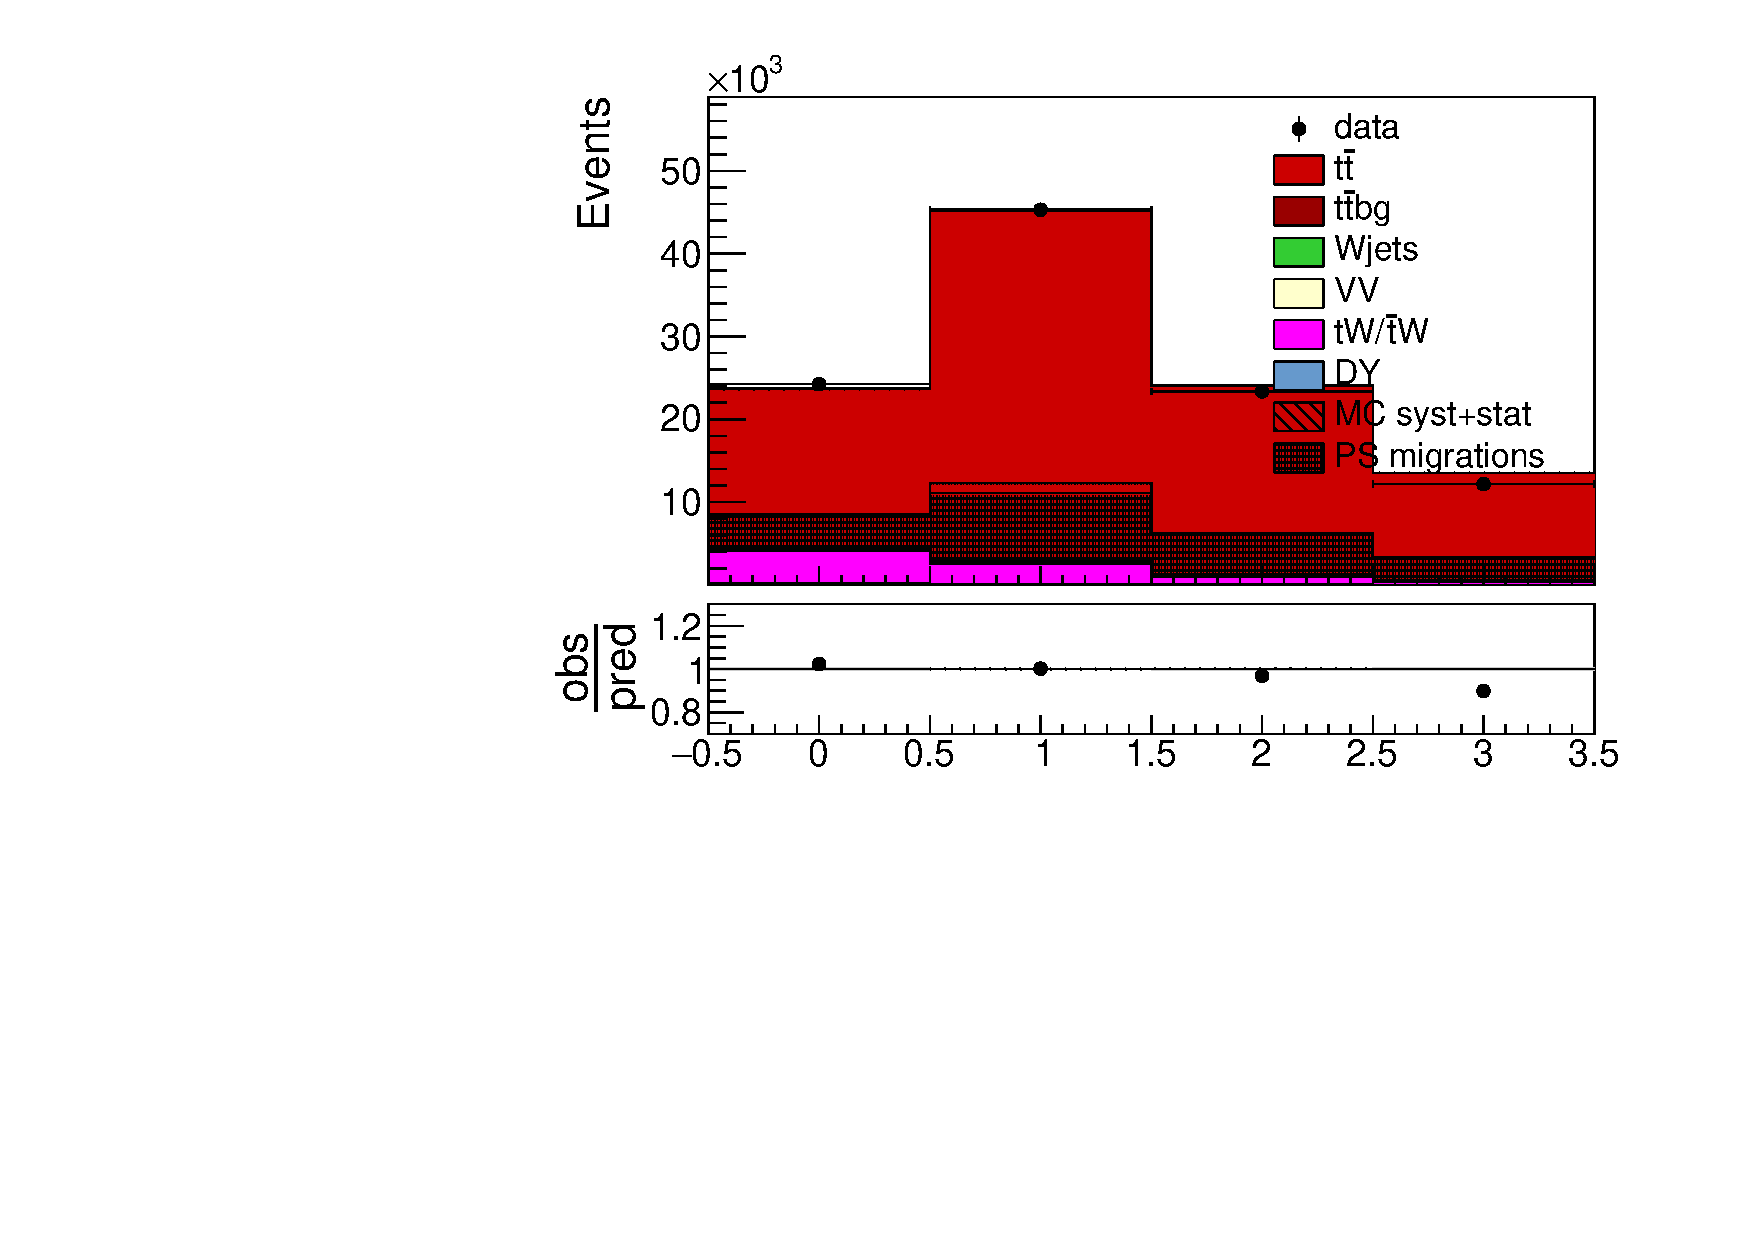
\includegraphics{SystematicUncerts/Figures/variationPlots/controlPlots/TT_MESCALE/jet_multi_1x_b-jets_step_8_TT_MESCALE_down.pdf}}
    \resizebox{0.48 \textwidth}{!}{\includegraphics{SystematicUncerts/Figures/variationPlots/controlPlots/TT_MESCALE/jet_multi_1x_b-jets_step_8_nominal.pdf}}
    \resizebox{0.48 \textwidth}{!}{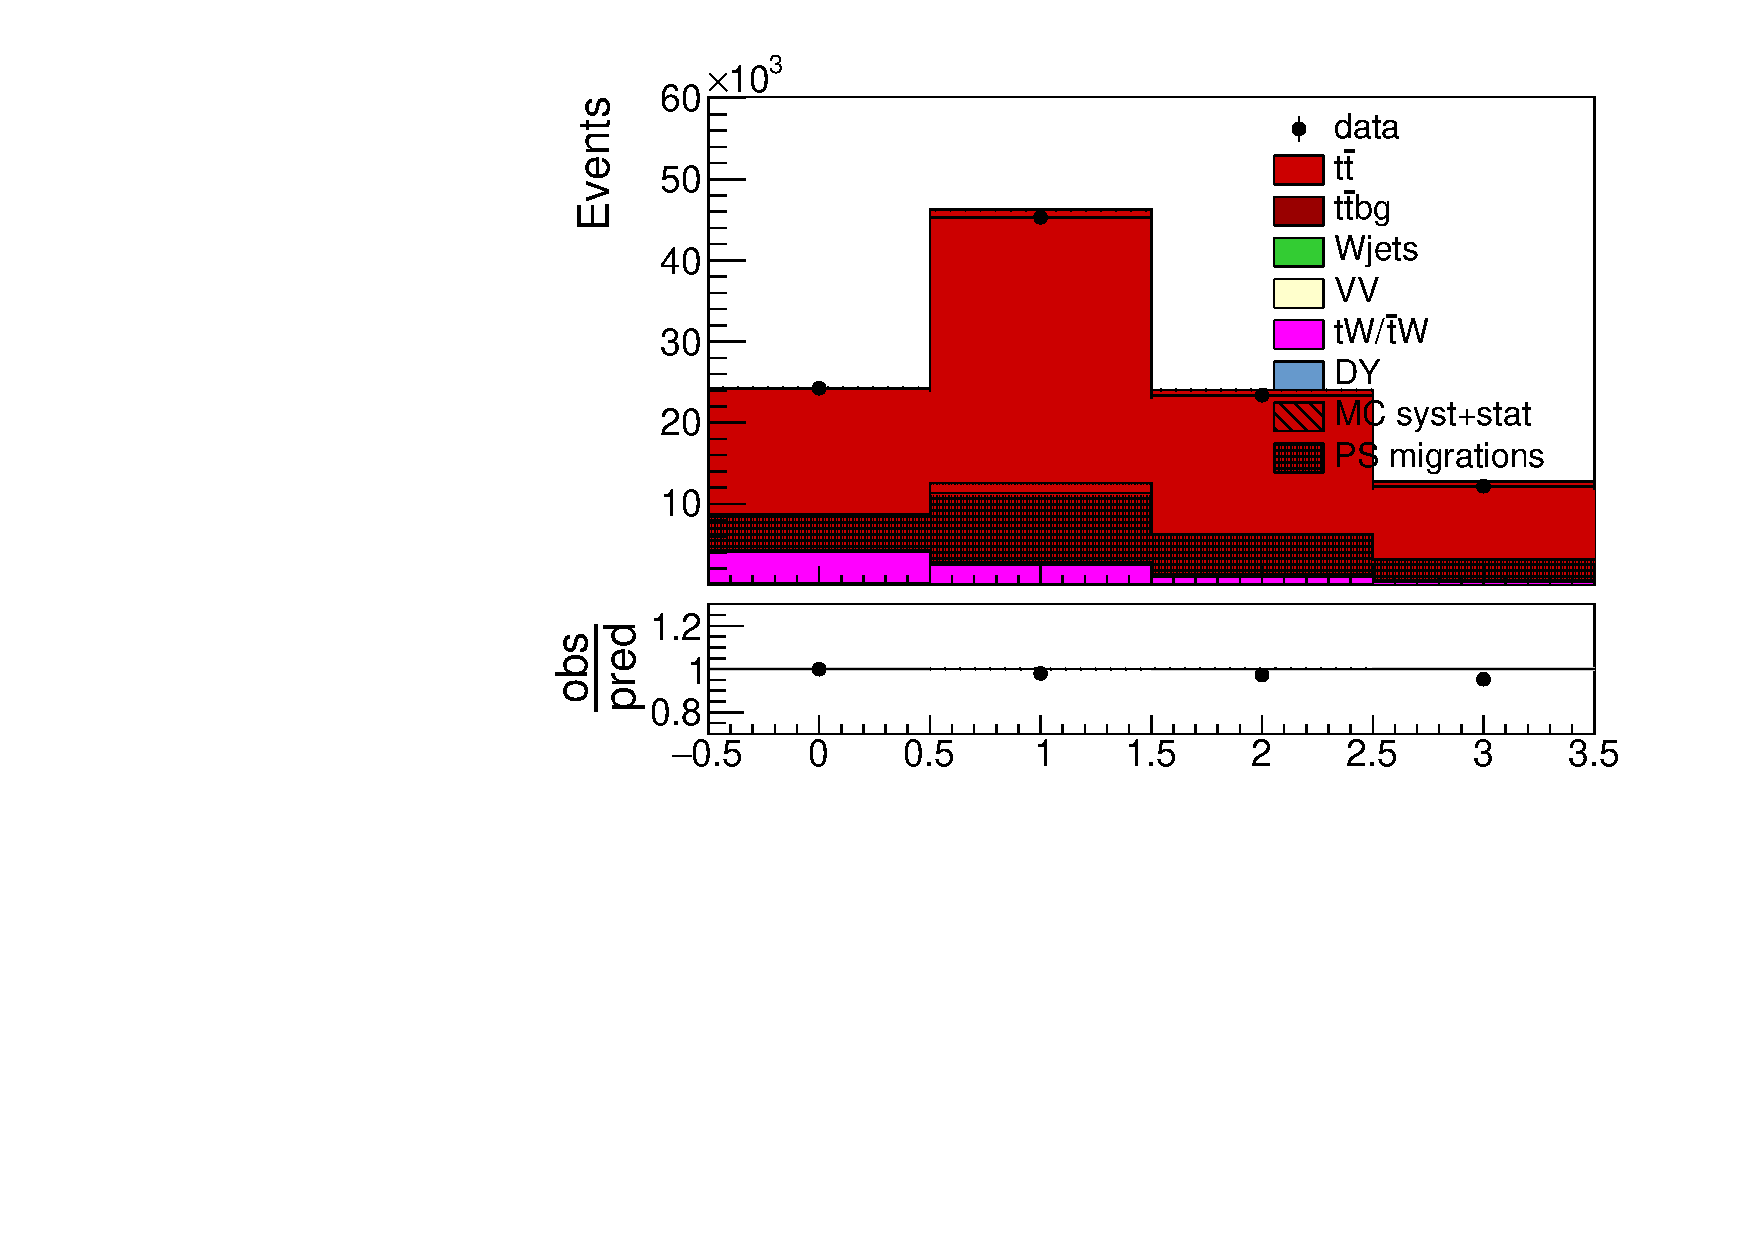
\includegraphics{SystematicUncerts/Figures/variationPlots/controlPlots/TT_MESCALE/jet_multi_1x_b-jets_step_8_TT_MESCALE_up.pdf}}
\caption{Number of additional jets for events with one b-tagged jet in the \emu channel for the two systematic variations (left, right) and the nominal \ttbar matrix element scale.
The hatched bands correspond to the statistical uncertainty on the sum of the predicted yields. 
        The ratios of the event yield in data to the sum of the predicted yields are
        shown at the bottom of each plot. Here, the solid gray band
        represents the contribution of the statistical uncertainty.
  \label{fig:control_var_TT_MESCALE}}
  \end{center}
\end{figure}

A similar uncertainty is applied to the scale of the parton shower calculations as modeled by \PYTHIA, split between the scale parameter impacting initial state radiation (ISR) and final state radiation (FSR). 
For the ISR scale the parameter is again varied by a factor of $2$ and $0.5$ respectively. The FSR scale parameter is varied by a factor of $\sqrt{2}$ or $\sqrt{0.5}$, following the recommendation
in Reference\cite{Skands:2014pea}. 
These uncertainties should also cover uncertainties on the detector response. Possible correlations between these theoretical uncertainties and  experimental uncertainties 
are taken into account by fitting all nuisance parameters simultaneously.
Figures \ref{fig:control_var_TT_ISRSCALE}
and \ref{fig:control_var_TT_FSRSCALE} show the variations to ISR and FSR respectively for the distribution of the number of additional jets for events with one b-tagged jet in the \emu channel.
Up to three jets can originate from particles generated in the matrix element calculations, so the impact of any changes in the parton shower scale are best seen in events with three or additional jets.
The plots also show a change in general normalisation because events migrate between the different categories for the number of b-tagged jets.

\begin{figure}[htbp!]
  \begin{center}
      \resizebox{0.48 \textwidth}{!}{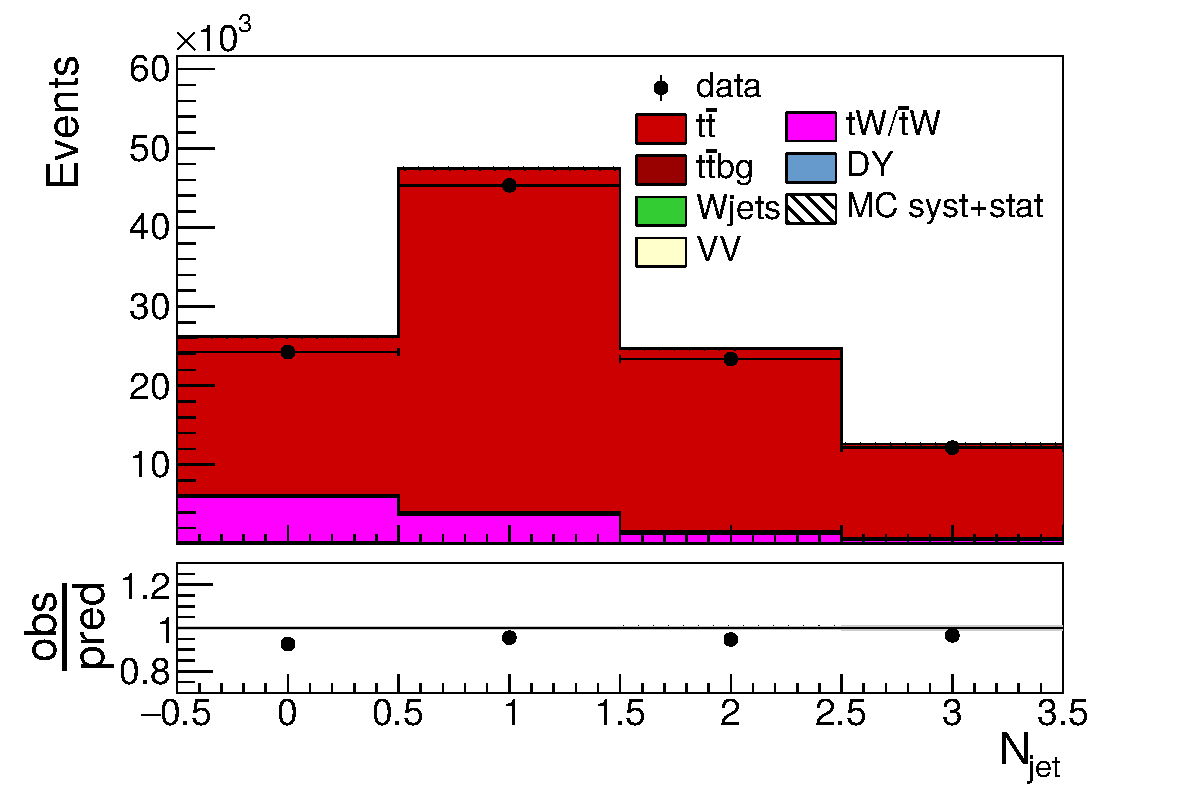
\includegraphics{SystematicUncerts/Figures/variationPlots/controlPlots/TT_ISRSCALE/jet_multi_1x_b-jets_step_8_TT_ISRSCALE_down.pdf}}
    \resizebox{0.48 \textwidth}{!}{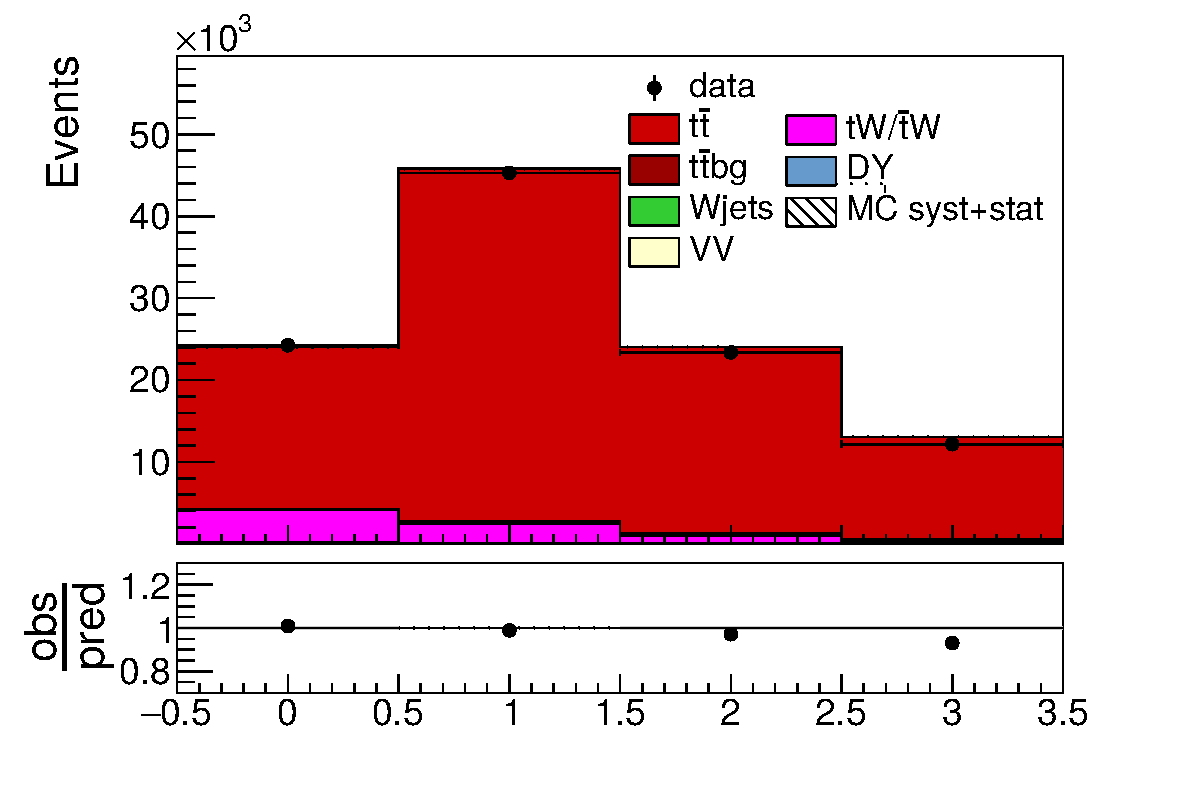
\includegraphics{SystematicUncerts/Figures/variationPlots/controlPlots/TT_ISRSCALE/jet_multi_1x_b-jets_step_8_nominal.pdf}}
    \resizebox{0.48 \textwidth}{!}{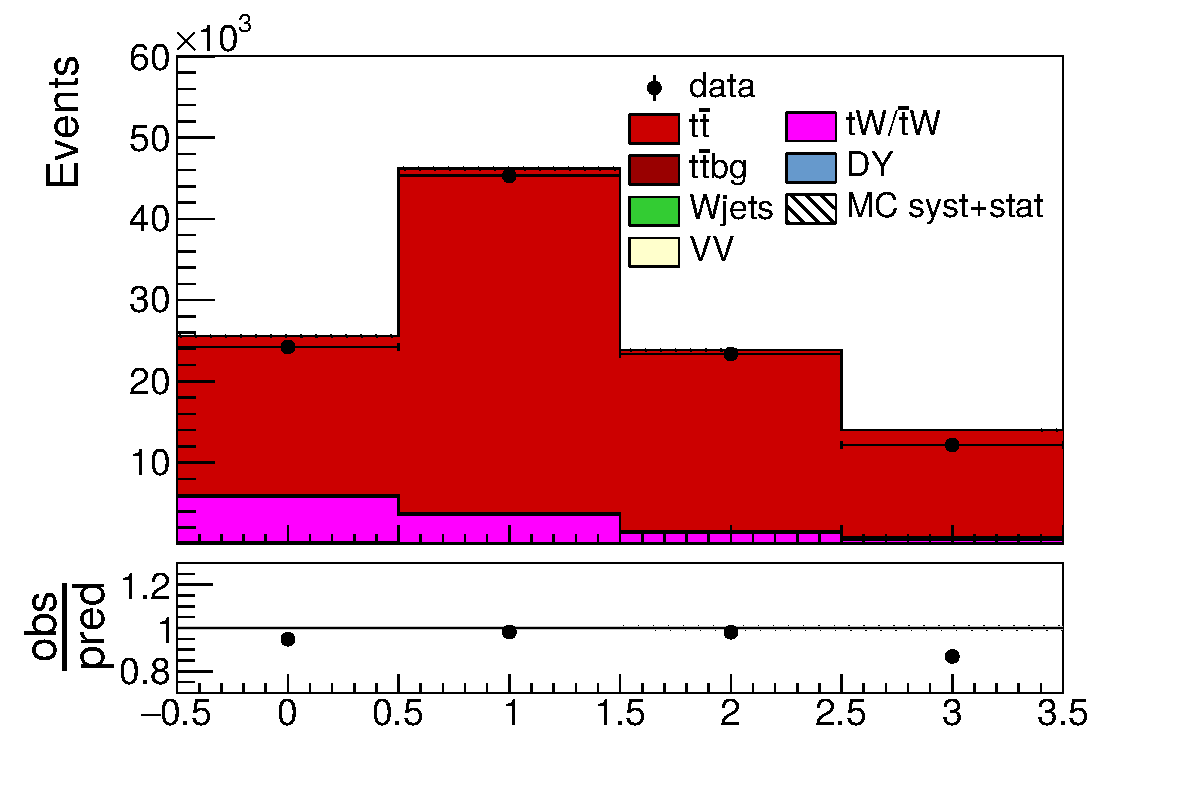
\includegraphics{SystematicUncerts/Figures/variationPlots/controlPlots/TT_ISRSCALE/jet_multi_1x_b-jets_step_8_TT_ISRSCALE_up.pdf}}
\caption{Number of additional jets for events with one b-tagged jet in the \emu channel for the two systematic variations (left, right) and the nominal ISR scale.
The hatched bands correspond to the statistical uncertainty on the sum of the predicted yields. 
        The ratios of the event yield in data to the sum of the predicted yields are
        shown at the bottom of each plot. Here, the solid gray band
        represents the contribution of the statistical uncertainty
  \label{fig:control_var_TT_ISRSCALE}}
  \end{center}
\end{figure}

\begin{figure}[htbp!]
  \begin{center}
      \resizebox{0.48 \textwidth}{!}{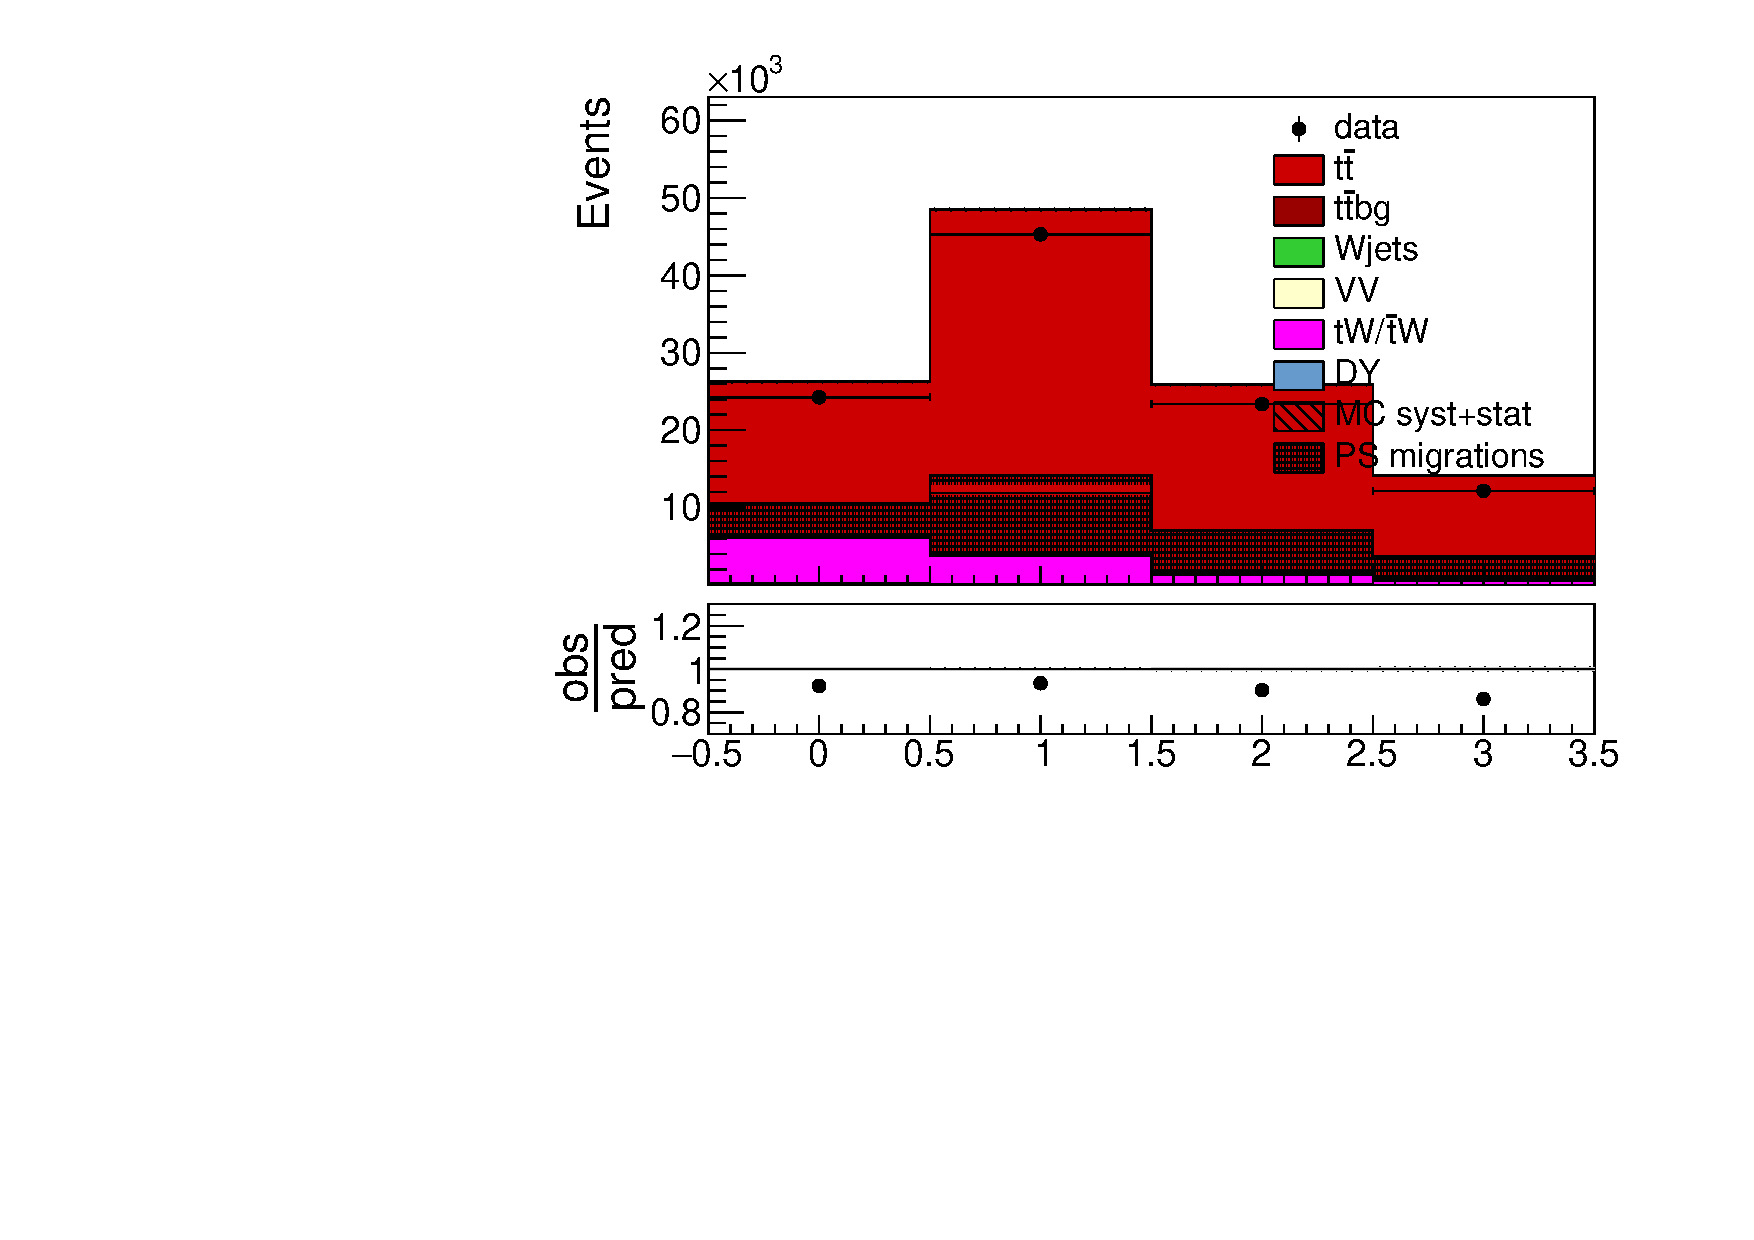
\includegraphics{SystematicUncerts/Figures/variationPlots/controlPlots/TT_FSRSCALE/jet_multi_1x_b-jets_step_8_TT_FSRSCALE_down.pdf}}
    \resizebox{0.48 \textwidth}{!}{\includegraphics{SystematicUncerts/Figures/variationPlots/controlPlots/TT_FSRSCALE/jet_multi_1x_b-jets_step_8_nominal.pdf}}
    \resizebox{0.48 \textwidth}{!}{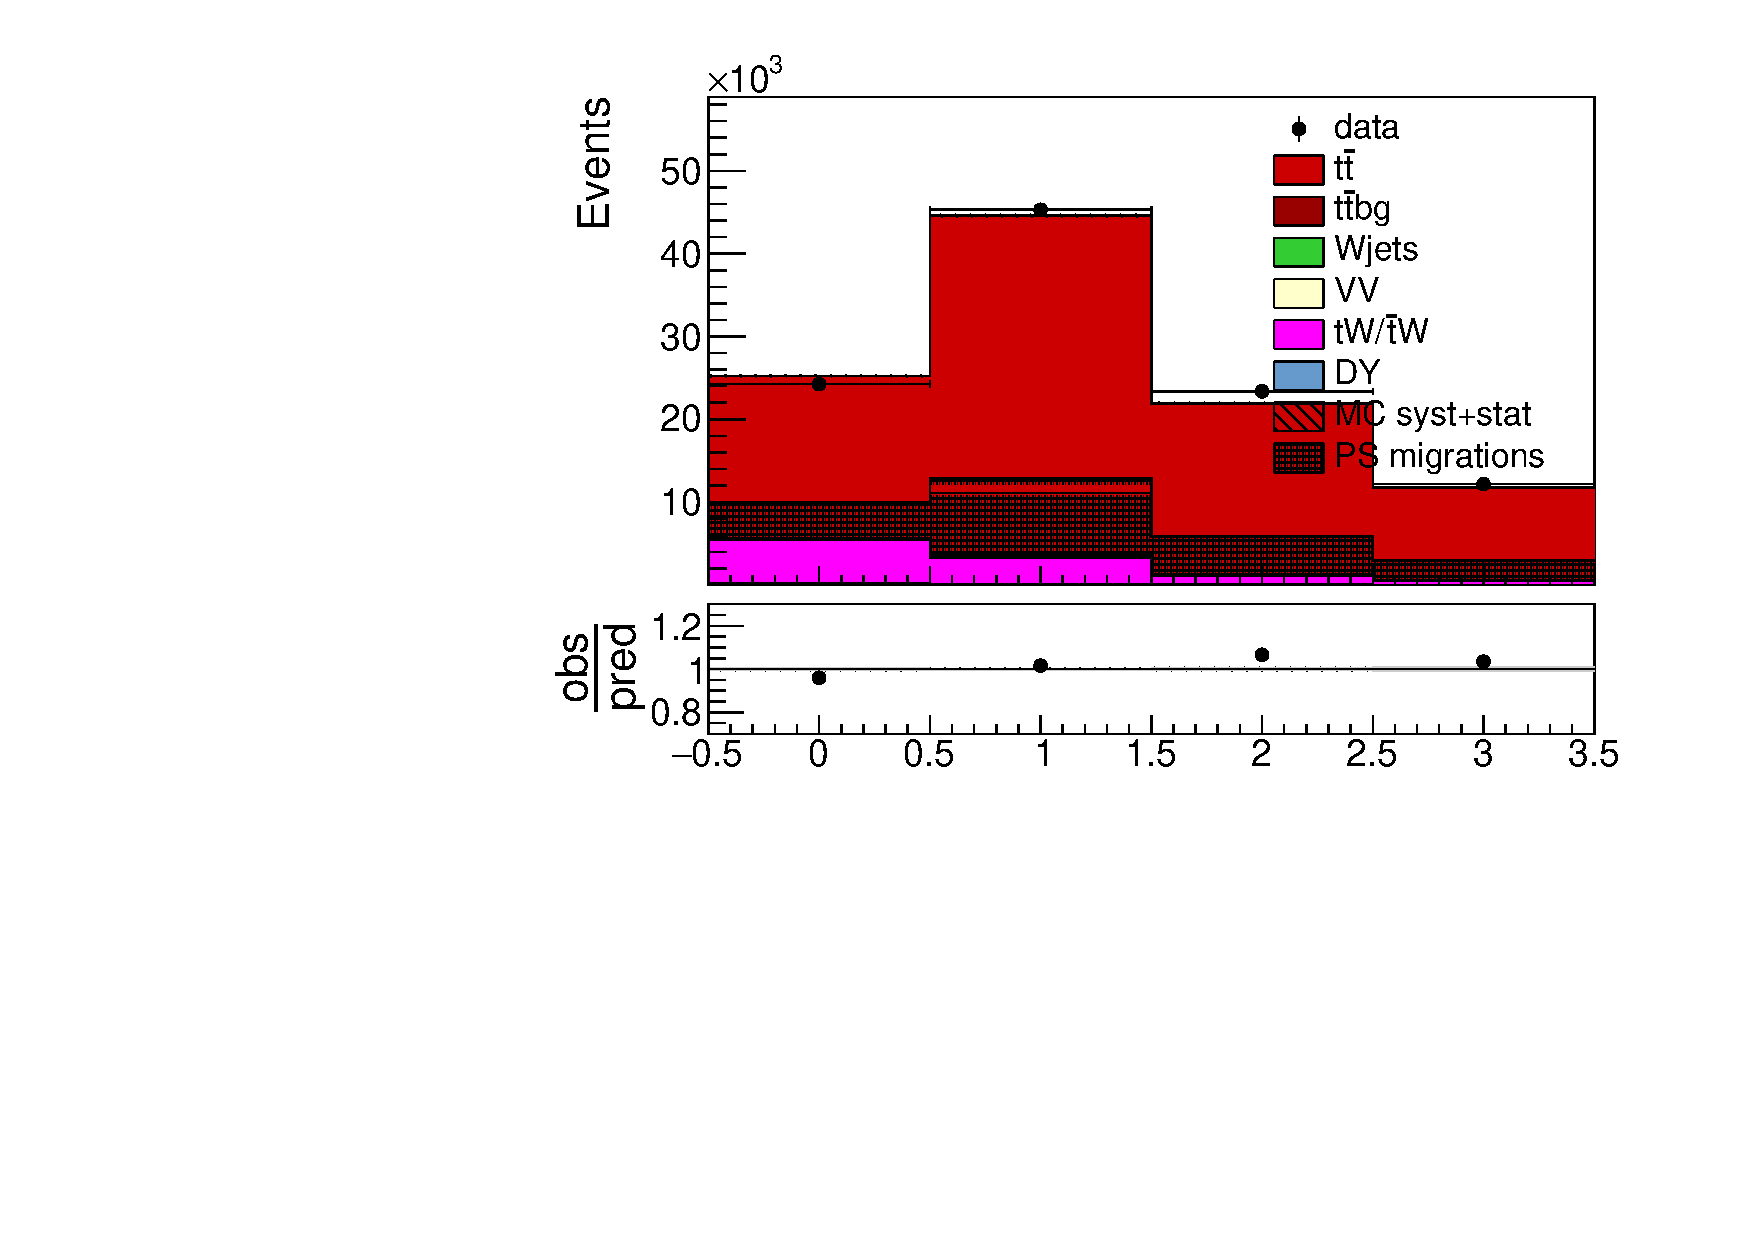
\includegraphics{SystematicUncerts/Figures/variationPlots/controlPlots/TT_FSRSCALE/jet_multi_1x_b-jets_step_8_TT_FSRSCALE_up.pdf}}
\caption{Number of additional jets for events with one b-tagged jet in the \emu channel for the two systematic variations (left, right) and the nominal FSR scale.
The hatched bands correspond to the statistical uncertainty on the sum of the predicted yields. 
        The ratios of the event yield in data to the sum of the predicted yields are
        shown at the bottom of each plot. Here, the solid gray band
        represents the contribution of the statistical uncertainty
  \label{fig:control_var_TT_FSRSCALE}}
  \end{center}
\end{figure}


In order to avoid overlap between particles generated in \POWHEG and \PYTHIA the emissions generated in Powheg are dampened according to the parameter $h_{damp}$ by a factor of $h_{damp}^2 / (h_{damp}^2 + \pt^2)$.
To obtain the systematic variations $h_{damp}$ is varied within it's uncertainty of $h_{damp} = 1.58^{+0.66}_{-0.59} m_t$
as determined by measurements using data taken by CMS at a center of mass energy of 8 TeV \cite{CMS-PAS-TOP-16-021}.

The simulation of the underlying event is tuned to data measured by CMS \cite{CMS-PAS-TOP-16-021}. The uncertainty from that tuning is propagated to the simulation resulting in a two sided variation.

The dependence on the model of color reconnection used for the hadronization in \PYTHIA is evaluated by comparing the nominal simulation with three different models \cite{Argyropoulos:2014zoa,Christiansen:2015yqa}. This results in three one-sided variations.

Differential measurements of the \ttbar cross section \cite{CMS-PAS-TOP-16-011} have shown that the simulation does not fully model the \pt distribution of the top quarks.
This is likely due to higher order effects as shown by differential NNLO calculations \cite{PhysRevLett.116.082003}. In order to model that disagreement a one-sided variation is introduced where simulated events are reweighted according to the \pt of the top quark with a factor of $\sqrt{SF(t)SF(\bar{t})}$ with $SF(\pt)=e^{0.0615-0.0005\cdot \pt}$.
This reweighting corrects the simulation to the measurement.

The uncertainty from the choice of PDF is evaluated using the variations provided by the CT14 PDF set \cite{Dulat:2015mca}. Uncorrelated variations are constructed from the central CT14 result using 56 eigenvectors resulting in 28 two-sided variations.
The variations are used at the $68 \;\%$ confidence level. Each of the variations is treated as a separate nuisance parameter.


The branching ratio of B mesons in \PYTHIA does not exactly agree with the values from the PDG  \todo{cite}. Especially a semi-leptonic decay of the B meson causes a different detector response compared to a hadronic decay,
which propagates to a differently reconstructed b-jet introducing an uncertainty.
This uncertainty is modelled by reweighting the events so that the branching ratio in simulation agrees with the one in the PDG and the uncertainties on the prediction serve as systematic
variations. These variations are given a uniform nuisance parameter.

The momentum transfer from the b-quark to the B meson (fragmentation function) is controlled by \PYTHIA and can influence the kinematics of the reconstructed b-jet. 
The default modelling uses the Bowler-Lund model \cite{Bowler1981} with the parameter of $StringZ:rFactB = 0.855$ \cite{Skands:2014pea,CMS-PAS-TOP-16-021}.
The respective parameter is tuned to LEP data and its uncertainty is used as a systematic variation, resulting in $StringZ:rFactB = 0.855^{+0.224}_{-0.157}$.
The Peterson fragmentation function \cite{PhysRevD.27.105} is used as an additional one-sided variation. 

\section{Summary}

\begin{table}[htbp!]
\begin{center}
\caption{Table of the systematic uncertainties giving the name of the systematic as well as a short summary.
The dominant effect of the systematic uncertainty describes whether it has more of an effect on the shape or on the normalization.
The prior describes the chosen probability density function for the nuisance parameter.~\label{tab:syst_sum}}
\begin{tabular}{l|l|l|l}
Uncertainty                           & Dominant Effect    & Prior    &   Short description                  \\
\hline
\multicolumn{4}{l}{Experimental Uncertainties}                                                     \\
\hline
Electron efficiency                   & Normalization      & Gaussian & $0.5\%-2\%$  on electron scale factor \\
Muon efficiency                       & Normalization      & Gaussian & $1.25\%$ on muon scale factor  \\
Electron energy                       & Shape              & Gaussian & $\leq 0.5\%$ on electron energy \\
Muon energy                           & Shape              & Gaussian & $0.05\%-0.2\%$ on muon energy \\
Trigger efficiency                    & Normalization      & Gaussian & $\leq 0.5\%$ on trigger scale factor \\
Jet energy scale (JES)                & Shape              & Gaussian & 19 sources, $1\%-2\%$ total \\
Jet energy resolution (JER)           & Shape              & Gaussian & $1\%-5\%$ on resolution        \\
b-tagging efficiency                  & Shape              & Gaussian & $2\%-6\%$ on scale factor      \\
Pile-up                               & Shape              & Gaussian & $4.6\%$ on inelastic pp cross section \\
Luminosity                            & Normalization      & Gaussian & $2.6\%$ on integrated luminosity \\
\hline
\multicolumn{4}{l}{Theoretical Uncertainties}                                                     \\
\hline
Matrix element scale                  & Shape              & Uniform  & $\times 2\setminus0.5$ variation of $\mu_R\setminus\mu_F$ \\ 
ISR scale                             & Shape              & Uniform  & $\times 2\setminus0.5$ variation of ISR scale \\
FSR scale                             & Shape              & Uniform  & $\times \sqrt{2}\setminus\sqrt{0.5}$ variation of ISR scale \\ 
Matching                              & Shape              & Gaussian & $h_{damp} = 1.58^{+0.66}_{-0.59} m_t$ in \POWHEG \\
Color Reconnection                    & Shape              & Gaussian & 3 models, one sided \\
Top \pt                               & Shape              & Uniform  & $SF(\pt)=e^{0.0615-0.0005\cdot \pt}$ one sided \\
PDF                                   & Shape              & Gaussian & 56 Eigenvectors from CT14 \\
B Meson BR                            & Shape              & Uniform  & semi leptonic br reweighted to PDG value \\
B Meson fragmentation                 & Shape              & Gaussian & $StringZ:rFactB = 0.855^{+0.224}_{-0.157}$ in \PYTHIA \\
\end{tabular}
\end{center}
\end{table}


